% This template is designed to be used with the `article' class, and was developed using MikTex 2.9.
\documentclass[12pt,letter]{article}

% poma_style.sty is used to generate the appropriate format
\usepackage{poma_style}

% Include any other packages and definitions needed
\usepackage{graphicx}
\usepackage{amsmath,amsfonts,bm}
\usepackage{courier}
\usepackage{titletoc}
\usepackage{lipsum}

\newcommand{\eps}{\varepsilon}
% DRAFT WATERMARK
	% NOTE: Comment out these two lines to remove watermark
    \usepackage[firstpage]{draftwatermark} % adds draft watermark
    \SetWatermarkLightness{0.85}

\begin{document}
%--------------------------------------------------------%
%	COVER PAGE
%--------------------------------------------------------%

\begin{titlepage}

  \newcommand{\HRule}{\rule{\linewidth}{0.5mm}} % Defines a new command for the horizontal lines, change thickness here

  \center % Center everything on the page


%	HEADING SECTION

  %\textsc{\LARGE University Name}\\[1.5cm] % Name of your university/college
  \textsc{\Large Simons Observatory Cryostat RFP}\\[0.5cm] % Major heading such as course name
  %\textsc{\large The Journal of Blah Blah}\\[0.5cm] % Minor heading such as course title

%	TITLE SECTION

  \vspace{1.5 cm}
  \HRule \\[0.4cm]
  { \huge \bfseries The Simons Observatory\\ Cryogenic Receiver RFP}\\[0.4cm] % Title of your document
  \HRule \\[1.5cm]
 
%	AUTHOR SECTION

  University of California, San Diego\\
  RFP \# SOCryo2017\\
  \vspace{.5 cm}
  {\it RFP Date:}\\
  \vspace{.5 cm}
  {\it Proposals Due:}\\


\vfill % Fill the rest of the page with whitespace

\end{titlepage}

%-----------------------------------------------------------------

\newpage

\tableofcontents
\clearpage

\section{General Information and Instructions}
The Simons Observatory collaboration is soliciting proposals for the design, fabrication, and testing of a liquid cryogen-free camera that will be mounted on a new telescope sited on the side of Cerro Toco in the Atacama region of Chile (latitude: 22.9581 deg South, longitude 67.7858 deg West) at an altitude of 5200 meters (For more information about the project see http://simonsobservatory.org/). The new polarization camera, Th Simons Observatory Large Aperture Receiver (SOLAR) will use Transition Edge Superconductor (TES) bolometers cooled to 100 mK. SOLAR will have a design similar to the existing ACTPol and Simons Array cameras which are currently operating at the Simons Observatory site. The cameras are designed to make sensitive observations of the Cosmic Microwave Background (CMB) at wavelengths between 0.9 mm and 3 mm. Simons Observatory is funded by the Simons Foundation.

This request for proposal consists of three sections plus appendices. The sections include the following:
\begin{enumerate}
\item General information and instructions — information about the project and the proposal process (this section).
\item Content of proposal — information about the format and content of the submitted proposal.
\item Specifications and statement of work — information about the design criteria and telescope performance requirements.
\end{enumerate}

The appendices include various representation, certification, acknowledgment, and signature forms.

\subsection{Institutional Management Structure}

\subsection{Form of proposal and manner of submission}

\subsection{Method of procurement}

\subsection{Criteria for Proposal Evaluation}
\subsection{Action Upon Proposals}
\subsection{No-bids}
\subsection{Questions}

\section{CONTENT OF PROPOSAL}
\subsection{Proposal format}
\subsection{General summary}
\subsection{Technical proposal}
	\subsubsection{Design}
    \subsubsection{Manufacturing Plan}
    \subsubsection{Pre-shipment Verification and Shipping Plan}
    \subsubsection{Assembly Plan}
    \subsubsection{Final Verification Plan}
    \subsubsection{Exceptions to SO specifications}
\subsection{Management}
\subsection{Summary schedules}
\subsection{Pricing}

\section{SO Specifications and Statement of Work}
\subsection{Statement of work}
	\subsubsection{General statement of work}
    The work described herein shall consist of the furnishing of labor, materials, services, drawings, data, detailed specifications, test documents and other items required for the detailed design, manufacture, and testing of SOLAR.
    
    \subsubsection{Objectives of the program}
    The primary objectives of the program concern the design, fabrication, assembly, and acceptance testing of SOLAR. The requirements are as follows:
    \begin{enumerate}
    \item {\it Driving Requirements}
    	\begin{enumerate}
        \item {\bf Optics Tubes} SOLAR will have ??? optics tubes which will hold filters, lenses, the detector arrays, and other optical components. SO will provide the detailed optical design, the lenses, filters and the detectors. The Vendor will be responsible for the design and manufacture of the mounts for these components to the specified tolerances. The optics tube manufacture and mounting in SOLAR must take into account thermal contraction, gravitational sag, and thermal conductivity to various components. The resonant frequencies of the optics tube should be greater than 20 Hz.
        \item {\bf Cryogenics} The detector arrays must run at 0.1K or below. The optical components will run at 4K. SO will provide estimates of thermal load from the detectors at 0.1K. There is also a significant load from cryogenic cabling required to run the detectors. While sample calculations of the loading from the cabling will be provided, the final number will depend on the Vendor routing and heat-sinking. Finally, the design of the mechanical mounts must be a balance between rigidity, strength and thermal load. 
        \item {\bf Magnetic Shielding Design} The cryogenic amplifiers for the detector arrays are extremely sensitive to magnetic fields. Magnetic shielding of the optics tubes is usually achieved with several tubular layers of high permeability material. The 4 K shielding is achieved with concentric cylinders of Cryoperm (Amuneal Manufacturing Corp.). There may be additional layers of Niobium shielding at 4 K and a large 300 K Mu-metal (Nickel-Iron alloy) shield around much of SOLAR. The SO collaboration has experience with this type of design and will provide existing drawings and calculations.
        \item {\bf Mechanical Compatibility} SOLAR must prescribe to an interface control document that will dictate how it couples to the overall telescope structure.
        \item {\bf Design Appropriateness} The working space must be reasonably accessible for installation and maintenance of the cryogenic components. SOLAR will be shipped to the high mountains of Chile and installed on the SO telescope, so it must be robustly designed so that it is not easily damaged by these activities.
        \end{enumerate}
    \item
    \item
    \item
    \item
    \end{enumerate}
    \subsubsection{Summary of Vendor deliverables}
    \subsubsection{Kickoff System Requirement Review (SRR)}
    \subsubsection{Preliminary Design Review (PDR)}
    \subsubsection{Critical Design Review (CDR)}
    \subsubsection{Complete Design Documentation (CDD)}
\subsection{Design constraints}   

    \subsubsection{SO Configuration}
    
    SOLAR is a ??? frequency camera designed to interface with a SO large aperture telescope. A preliminary optics layout for the telescope is shown in ???. We anticipate that the final design will be very close to what is shown in this figure. It consists of ??? separate optics tubes comprised of three SO provided ??? lenses, three to five SO provided plastic mesh filters, a Lyot stop, magnetic shielding, and an SO provided detector array. The main mechanical interface is anticipated to be a “cold plate” maintained at 3-4 K by one or more pulse tube coolers. The SO provided windows are made from ???. The anticipated tolerance of the mounting of the main components (lenses and detector arrays) is expected to be approximately 500 microns in order to maintain the required image quality. The readout electronics mounted on the detector arrays is extremely susceptible to magnetic fields. The optics tubes must therefore be shielded with several layers of Cryoperm magnetic shielding (see ???).
    
The detectors are designed to operate at 100 mK. Therefore we anticipate the need for a dilution refrigerator system. The exact cryogenic design will be determined by the Vendor in consultation with SO. However, for the purposes of this RFP we offer some design parameters to help the Vendor with their proposal....???

The Vendor-supplied thermometry and cables are required for the cryogenic operation of SOLAR. However, they also provide crucial information for understanding the health and operation of the detectors and ultimately the quality of the data. Therefore the Vendor will install thermometers throughout the system. SO anticipates the need for ??? total thermometers mounted to the various optical components, refrigerator stages, and cold electronics. The thermometry will be a mixture of diodes (e.g. Lakeshore DT570) and ROXs. The Vendor will supply the thermometers as well as the cabling while the SO project will provide the thermometry read-out electronics.

Readout wires???

    \subsubsection{Operating Conditions}
    
    SOLAR will be operating on a SO telescope located at an altitude of 5200 meter in Northern Chile. SOLAR will be optically aligned and rigidly mounted inside the telescope receiver cabin. However, the entire telescope scans in both azimuth and elevation. In particular, the azimuth scan moves the telescope +/- 3 degree in a triangle scan with a period of 8 seconds. The maximum acceleration is 10 deg/s2. SOLAR is located near the axis of rotation, so the translation is limited to the physical size of SOLAR. However, care must be taken to make the system resistant both mechanically and cryogenically to these motions. All of the cables must be mechanically secured to prevent motion during the scan.
    
\subsection{Performance requirements}
    \subsubsection{Optical}
    \subsubsection{Cryogenic Performance}
    \subsubsection{Mechanical}
    \subsubsection{Access and reliability}
\subsection{Materials and fabrication}
\subsection{Drawings, specifications and tests}
    \subsubsection{Design and manufacturing drawings}
    \subsubsection{Design calculations and data}
    \subsubsection{Assembly, alignment and test plans}
    \subsubsection{Test instrumentation}
    \subsubsection{Quality assurance and inspection}
    \subsubsection{Operation and maintenance manuals}
    \subsubsection{Spare parts}
\subsection{Summary of Deliverables and Specifications}
\subsection{Summary of ACT Supplied Parts}
\subsection{Summary of the ACT Project and Vendor Interfaces}
    \subsubsection{Technical}
    \subsubsection{Management}

\appendix

\section*{Appendix A}

\begin{itemize}
	\item Present their work in clear, grammatically correct English
	\item Lay out the camera-ready manuscript in a professional manner
	\item Ensure all figures are readable and attractive
	\item Provide adequate reference to prior literature used in the work
	\item Strive for technical correctness. While the level of review does not approach that of JASA, POMA does not intend to publish any paper where the initial premises, reported results, or conclusions are wrong. 
\end{itemize}

\begin{figure}
	\centering
	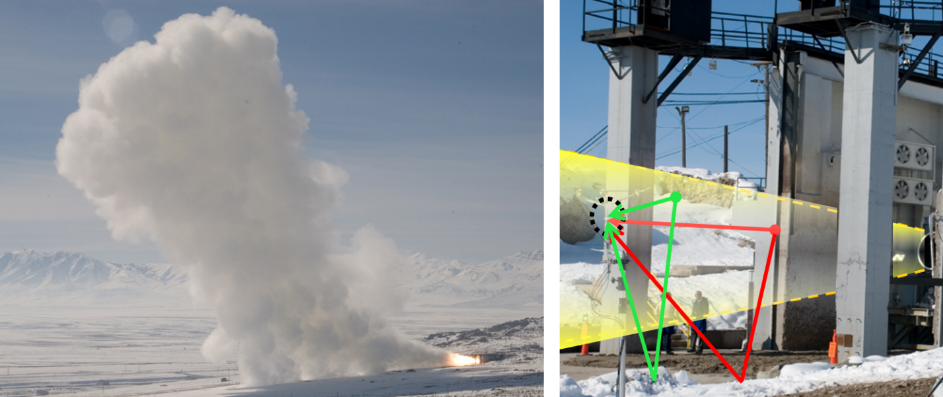
\includegraphics{GEM60_Picture}
	\caption{\label{fig:gem60}Distant view of a GEM-60 solid rocket motor firing.}
\end{figure}

\begin{table}
	\centering
	\caption{\label{tab:rocket}Sample rocket parameters.}
\begin{tabular}{lcl}
	\textbf{Parameter} & \textbf{Symbol} & \textbf{Value} \\ \hline
	Thrust & $T$ & 870 kN \\
	Diameter & $D$ & 1.2 m \\
	Centerline velocity & $v_j$ & 2000 m/s
\end{tabular}
\end{table}

\begin{equation}
	\Phi_{l,k_z}(r,\phi,z) \equiv \frac{H_l^{(1)}(k_rr)}{H_l^{(1)}(k_rr_0)} e^{il\phi}e^{ik_zz}, \hspace{10mm} r\ge r_0.
\end{equation}


\begin{enumerate}
	\item \textbf{Do not upload Word or .tex files to Editorial Manager.}
	\item \textbf{Cover page information (affiliations, etc.) must match author metadata.}
	\item \textbf{It is imperative that page size and margin requirements are followed.}
\end{enumerate}




\begin{thebibliography}{9}

\bibitem{daigle79}
	G. A. Daigle, ``Effects of atmospheric turbulence on the interference of sound waves above a finite impedance boundary'', \textsl{J. Acoust. Soc. Am.} \textbf{65}, 45-49 (1979).

\end{thebibliography}



\end{document}










































